\subsection{Häufige Parametrisierungen}
    \subsubsection{Ellipse}
    \vspace{0em}
    \mathbox{
        \overrightarrow{r}(t) = \binom{a \cdot cos(t) + x_0}{b \cdot sin(t) + y_0}
    }
    \text{Sonderfall Kreis mit Radius } a = b
    \begin{center}
        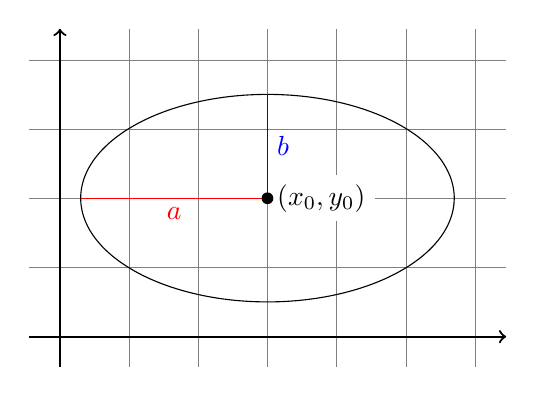
\begin{tikzpicture}[x=0.75pt,y=0.75pt,yscale=-1,xscale=1]
            %coordinatum system
            \foreach \i in {0, ..., 6} {
                \draw [very thin,gray] (\i * 33.33, -15) -- (\i * 33.33, 148);
            }
            \foreach \i in {0, ..., 4} {
                \draw [very thin,gray] (-15 ,\i * 33.33) -- (215 ,\i * 33.33);
            }
            \draw[thick, <-] (0, -15) -- (0, 148);
            \draw[thick, ->] (-15, 133.33) -- (215, 133.33);
            %
            %Ellipse
            \draw plot [smooth, samples = 100, domain = 0:500] ({90 * cos(\x) + 100}, {50 * sin(\x) + 66.6});
            %a
            \draw [red] (100, 66.66) -- (55, 66.66) node[anchor = north, red] {$a$} -- (10, 66.66);
            %b
            \draw [blue] (100, 66.66) -- (100, 41.66) node[anchor = west, blue] {$b$} -- (100, 16.66);
            %Midpoint
            \draw (100, 66.66) node[right, fill=white] {$(x_0, y_0)$} node[circle, fill, inner sep = 1.5pt]{};
        \end{tikzpicture}\\
    \end{center}
    
    \subsubsection{Zykloide}
    \vspace{0em}
    \mathbox{
        \overrightarrow{r}(t) = \binom{rt - a \sin(t)}{r - a \cos(t)}
    }
    \text{Sonderfall Gewöhnliche Zykloide } r = a\\
    \begin{center}
        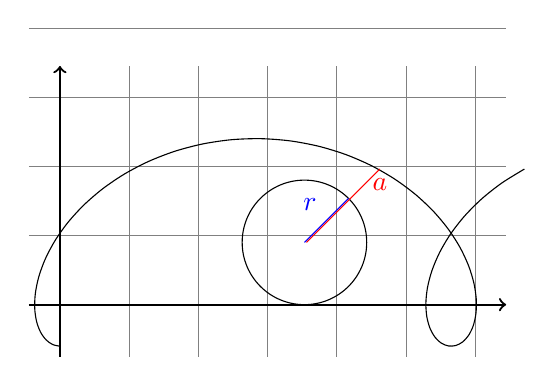
\begin{tikzpicture}[x=0.75pt,y=0.75pt,yscale=1,xscale=1]
            %coordinatum system
            \foreach \i in {0, ..., 6} {
                \draw [very thin,gray] (\i * 33.33, -25) -- (\i * 33.33, 115);
            }
            \foreach \i in {0, ..., 4} {
                \draw [very thin,gray] (-15 ,\i * 33.33) -- (215 ,\i * 33.33);
            }
            \draw[thick, ->] (0, -25) -- (0, 115);
            \draw[thick, ->] (-15, 0) -- (215, 0);
            %
            %Zykloide
            \draw plot [smooth, variable=\x, domain=0:2.75*pi, samples = 50] ({30 * \x - 50 * sin(\x*180/pi)},{30 - 50 * cos(\x*180/pi)});
            %circle
            \draw ({30 * (1.25 * pi)}, 30) circle (30);
            %a
            \draw [red] ({1 + 30 * (1.25 * pi)}, 30) -- ({1 + 30 * (1.25 * pi) - 50 * sin((1.25 * pi)*180/pi)}, {30 - 50 * cos((1.25 * pi)*180/pi)}) node[anchor = north, red] {$a$};
            %radius
            \draw [blue] ({30 * (1.25 * pi)}, 30) -- ({(30 * (1.25 * pi) + 30 * (1.25 * pi) + 30 * 1.414/2)/2}, {(30 + 30 + 30 * 1.414/2)/2}) node[anchor = south east, blue] {$r$} -- ({30 * (1.25 * pi) + 30 * 1.414/2}, {30 + 30 * 1.414/2});
            %
        \end{tikzpicture}\\
    \end{center}

    \subsubsection{Epizykloide}
    \vspace{0em}
    \mathbox{
        \overrightarrow{r}(t) = \binom{R cos(t) - a cos(\frac{R}{r} t)}{R sin(t) - a sin(\frac{R}{r} t)}
    }
    \text{Sonderfall Kardioide } R = 2r, r = a\\
    \begin{center}
        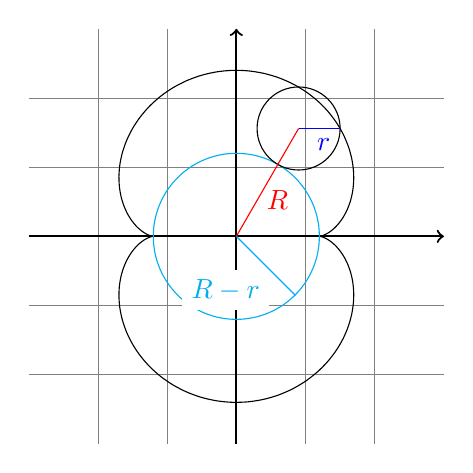
\begin{tikzpicture}[x=0.75pt,y=0.75pt,yscale=1,xscale=1]
            %coordinatum system
            \foreach \i in {-2, ..., 2} {
                \draw [very thin,gray] (\i * 33.33, -100) -- (\i * 33.33, 100);
            }
            \foreach \i in {-2, ..., 2} {
                \draw [very thin,gray] (-100 ,\i * 33.33) -- (100 ,\i * 33.33);
            }
            \draw[thick, ->] (0, -100) -- (0, 100);
            \draw[thick, ->] (-100, 0) -- (100, 0);
            %
            %Epizykloide
            \draw plot [smooth, variable=\x, domain=0:2*pi, samples = 100] ({60 * cos(\x*180/pi) - 20 * cos(60/20 * \x*180/pi)},{60 * sin(\x*180/pi) - 20 * sin(60/20 * \x*180/pi)});
            %big circle
            \draw [cyan] (0, 0) circle (40);
            \draw [cyan] (0, 0) -- (1.424/4 * 45, -1.424/4 * 45) node[anchor = north east, cyan, fill=white] {$R-r$} -- (1.424/2 * 40, -1.424/2 * 40);
            %small circle (t = pi/3)
            \draw ({60 * cos(60)}, {60 * sin(60)}) circle (20);
            %R
            \draw [red] (0, 0) -- ({20 * cos(60)}, {20 * sin(60)}) node[anchor = west, red] {$R$} -- ({60 * cos(60)}, {60 * sin(60)});
            %r
            \draw [blue] ({60 * cos(60)}, {60 * sin(60)}) -- ({60 * cos(60) - 20 * cos(60/20 * 60)},{60 * sin(60) - 20 * sin(60/20 * 60)}) node[anchor = north east, blue] {$r$};
            %
        \end{tikzpicture}\\
    \end{center}

    \subsubsection{Hypozykloide}
    \mathbox{
        \overrightarrow{r}(t) = \binom{R cos(t) + a cos(\frac{R}{r} t)}{R sin(t) - a sin(\frac{R}{r} t)}
    }
    \begin{center}
        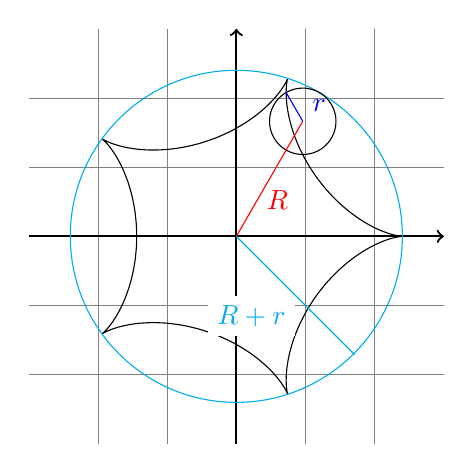
\begin{tikzpicture}[x=0.75pt,y=0.75pt,yscale=1,xscale=1]
            %coordinatum system
            \foreach \i in {-2, ..., 2} {
                \draw [very thin,gray] (\i * 33.33, -100) -- (\i * 33.33, 100);
            }
            \foreach \i in {-2, ..., 2} {
                \draw [very thin,gray] (-100 ,\i * 33.33) -- (100 ,\i * 33.33);
            }
            \draw[thick, ->] (0, -100) -- (0, 100);
            \draw[thick, ->] (-100, 0) -- (100, 0);
            %
            %Hypozykloide
            \draw plot [smooth, variable=\x, domain=0:2*pi, samples = 100] ({64 * cos(\x*180/pi) + 16 * cos(64/16 * \x*180/pi)},{64 * sin(\x*180/pi) - 16 * sin(64/16 * \x*180/pi)});
            %big circle
            \draw [cyan] (0, 0) circle (80);
            \draw [cyan] (0, 0) -- (1.424/4 * 80, -1.424/4 * 80) node[anchor = north east, cyan, fill=white] {$R+r$} -- (1.424/2 * 80, -1.424/2 * 80);
            %small circle (T = pi/3)
            \draw ({64 * cos(60)}, {64 * sin(60)}) circle (16);
            %R
            \draw [red] (0, 0) -- ({20 * cos(60)}, {20 * sin(60)}) node[anchor = west, red] {$R$} -- ({64 * cos(60)}, {64 * sin(60)});
            %r
            \draw [blue] ({64 * cos(60)}, {64 * sin(60)}) node[anchor = south west, blue] {$r$} -- ({64 * cos(60) + 16 * cos(64/16 * 60)},{64 * sin(60) - 16 * sin(64/16 * 60)});
            %
        \end{tikzpicture}\\
    \end{center}

    \subsubsection{Lissajous-Figuren}
    \mathbox{
        \overrightarrow{r}(t) = \binom{a_1 sin(\omega_1 t + \varphi_1)}{a_2 sin(\omega_2 t + \varphi_2)}
    }